\documentclass{article}
\usepackage{amsfonts, amsmath, amssymb, amsthm} % Math notations imported
\usepackage{enumitem}
\usepackage{graphicx}
\usepackage[margin=1in]{geometry}
\graphicspath{ {.} }

\newtheorem{thm}{Theorem}
\newtheorem{prop}[thm]{Proposition}
\newtheorem{cor}[thm]{Corollary}

% title information
\title{Math 180A HW0}
\author{Neo Lee}
\date{01/13/2023}

% main content
\begin{document} 

% placing title information; comment out if using fancyhdr
\maketitle 

\textbf{Problem 4} 
\begin{enumerate}[label=(\alph*)]
    \item 
    \begin{center}
        
        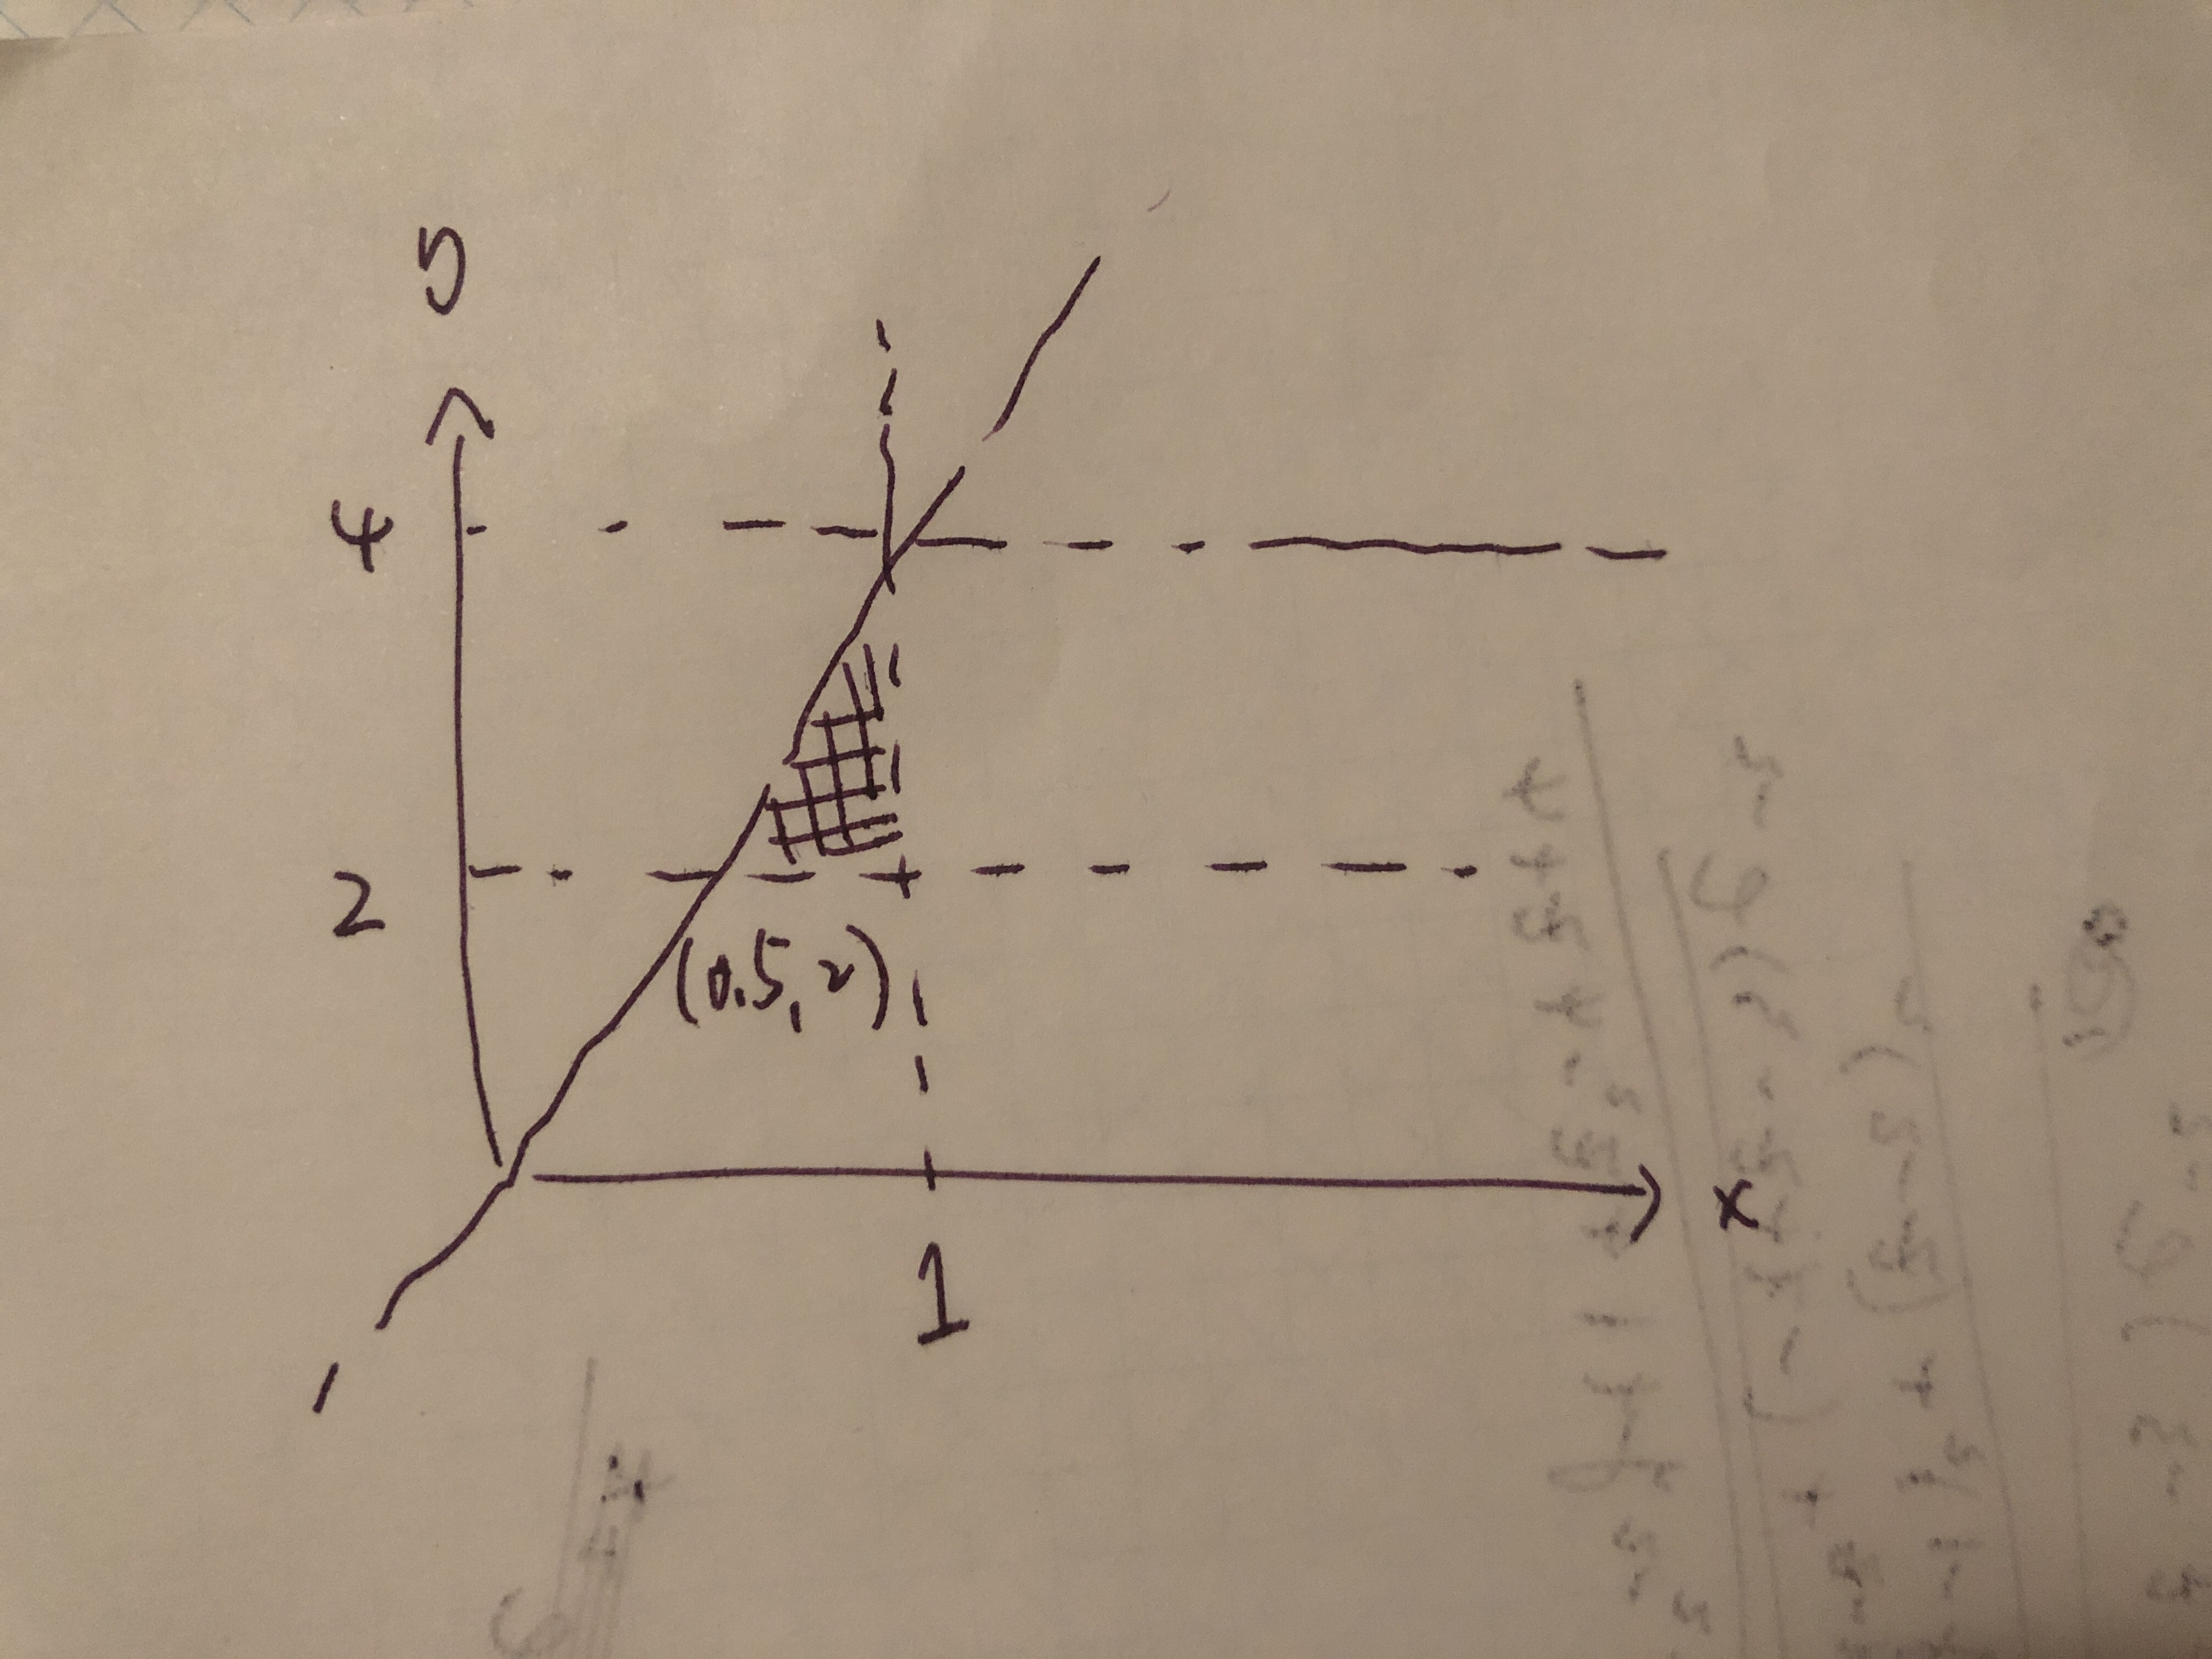
\includegraphics[width=0.7\textwidth]{Q4.jpg}
    \end{center}
    \item 
    \begin{align}
        \iint_{D}6xy^{2}dxdy &= \int_{2}^{4}\int_{0.5}^{1}6xy^{2}dxdy 
        \\ &= \int_{2}^{4} \int_{0.5}^{1} 6xy^{2} dxdy 
        \\ &= \int_{2}^{4} 3x^{2}y^{2} dy \Big|_{0.5}^{1}
        \\ &= \int_{2}^{4} \left(3y^{2}\right) - \left(0.75y^{2}\right) dy
        \\ &= \int_{2}^{4} 2.25y^{2} dy
        \\ &= 0.75y^{3} \Big|_{2}^{4}
        \\ &= 0.75 \cdot 4^{3} - 0.75 \cdot 2^{3}
        \\ &= 42
    \end{align} \\
\end{enumerate}
\smallskip


\textbf{Problem 5} 
\begin{enumerate}[label=(\alph*)]
    \item $A \cap B \cap C$
    \item $A \cap B^{c} \cap C^{c}$
    \item $A \cup B$
    \item $A \cap B \cap C^{c}$ 
\end{enumerate}
\smallskip

\textbf{Problem 6} 
\begin{enumerate}[label=(\alph*)]
    \item $2^{10}$
    \item $10 \choose 5$
\end{enumerate}
\smallskip

\textbf{Problem 7} 
\begin{enumerate}[label=(\alph*)]
    \item 
    \begin{align}
        \sum_{k=0}^{\infty} \frac{x^{2k}}{4^{k}} 
        &= \sum_{k=0}^{\infty} \left(\frac{x^2}{4}\right)^{k}
        \\ &= \frac{1}{1 - \frac{x^2}{4}}
    \end{align}
    \item 
    \begin{align}
        \sum_{k=0}^{\infty} \frac{x^{k + 1}}{k!} &= \sum_{k=0}^{\infty} \frac{x^{k}}{k!} \cdot x
        \\ &= x \cdot e^{x} 
    \end{align}
\end{enumerate}
    


\end{document}